\section{Diferencia entre el MaxEnt y el AssMap}


No tenemos ninguna razón para asegurar que el estado de máxima entropía y el estado asignado por promedio son el mismo. En la asignación promedio se hacen dos suposiciones fuertes: primero, que el sistema microscópico se halla en un estado puro (aunque no asigne un estado puro al estado efectivo). Segundo, que todos los estados puros son igualmente probables. Aunque estas suposiciones puedan parecer razonables, Jaynes, en su artículo, argumenta que estas no son tan arbitrarias como cualquier otra suposición, a menos que algún tipo de simetría del sistema sugiera lo contrario.

Nos preguntamos, pues, sobre la diferencia entre el estado de máxima entropía y el estado promedio. Calculamos, pues, la distancia entre estos estados como una función del parámetro $p_{1}$ de la aplicación de grano grueso (recuérdese que en el caso $n=1$ el segundo parámetro es simplemente $1-p_{1}$). Esto es, nos interesa obtener
\begin{equation}
    \text{d}\qty(\avgass(\rho_{\ef}),\maxass(\rho_{\ef}))=\text{d}\qty(\avgass(\rho_{\ef}),\maxass(\rho_{\ef}))(p_{1}),\nonumber
\end{equation}

\begin{figure}[ht!]
    \centering
      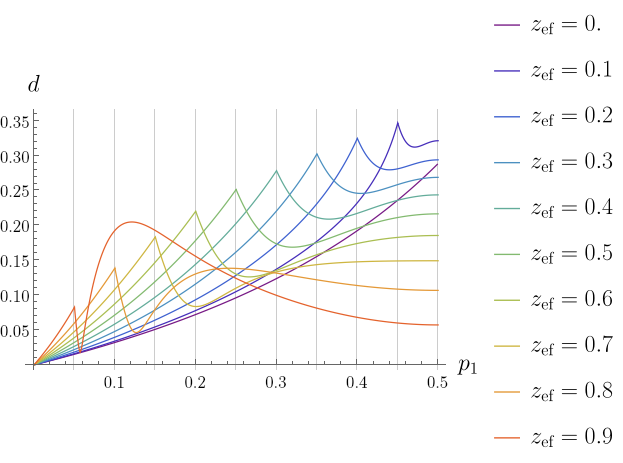
\includegraphics[width=0.9\linewidth]{chapter4/figures/maxavgdisr.png}
    \caption{Distancia entre asignaciones}
    \label{fig:AvgMaxDist}
\end{figure}

La figura  muestra que la fidelidad entre ambos estados parece constante siempre que $n>1000$, y que la verdadera dependencia se halla sobre el parámetro $p$. Veamos, pues, la fidelidad entre ambos estados como función de $p$, con $n=1000$.

La figura \ref{fig:AvgMaxDist} muestra que la distancia entre ambos estados para diferentes valores de $p_{1}$ y para diferentes valores de $r_{\ef}$. Como es natural, las asignaciones son la misma cuando el estado efectivo inicial es puro. En efecto, es sencillo demostrar que el único estado compatible con un estado efectivo inicial puro es $\rho_{\ef}^{\otimes n}$. Se ve, además, que las asignaciones coinciden también en el caso límite $p_{1}=1$ (y $p_{1}=0$ que es un caso límite únicamente cuando $n=2$).
